% Powered by Yujie He
% - https://github.com/hibetterheyj
% - yujie.he@epfl.ch
% - http://yujie-he.github.io/
% main structure borrowed from https://github.com/Denwid/pcml-cheatsheet
% new features
% - additional color hightlight
% - more compact style

\documentclass[10pt,a4paper,landscape]{article}
\usepackage{multicol}
\usepackage{calc}
\usepackage{ifthen}
\usepackage[landscape]{geometry}
\usepackage{amsmath,amsthm,amsfonts,amssymb,mathtools}
\usepackage{color,graphicx}
\usepackage{hyperref}
\usepackage{listings}
\usepackage{underscore}
\usepackage{todonotes}
\usepackage{graphicx}
% highlight
\usepackage{soul}
\soulregister\cite7
\soulregister\citep7
\soulregister\citet7
\soulregister\ref7
\soulregister\pageref7

\usepackage{comment}

% Cheatsheet style
% Cheatsheet style

% This sets page margins to .5 inch if using letter paper, and to 1cm
% if using A4 paper. (This probably isn't strictly necessary.)
% If using another size paper, use default 1cm margins.
\ifthenelse{\lengthtest{\paperwidth = 11in}}
  % Then
  { \geometry{top=.5in,left=.5in,right=.5in,bottom=.5in} }
  % Else
  { \ifthenelse{\lengthtest{\paperwidth = 297mm}}
	{\geometry{top=.4cm,left=.4cm,right=.4cm,bottom=.4cm} }
	{\geometry{top=.4cm,left=.4cm,right=.4cm,bottom=.4cm} }
  }

% Turn off header and footer
\pagestyle{empty}

% Redefine section commands to use less space
\makeatletter
%\renewcommand{\section}{\@startsection{section}{1}{0mm}%
%                                {-1ex plus -.5ex minus -.2ex}%
%                                {0.5ex plus .2ex}%x
%                                {\color{darkred}\normalfont\large\bfseries}}
%\renewcommand{\subsection}{\@startsection{subsection}{2}{0mm}%
%                                {-1explus -.5ex minus -.2ex}%
%                                {0.5ex plus .2ex}%
%                                {\color{darkdarkred}\normalfont\normalsize\bfseries}}
%\renewcommand{\subsubsection}{\@startsection{subsubsection}{3}{0mm}%
%                                {-1ex plus -.5ex minus -.2ex}%
%                                {1ex plus .2ex}%
%                                {\normalfont\small\bfseries}}
%%%%%% Section format
\usepackage[explicit]{titlesec}
\usepackage[many]{tcolorbox}
\titleformat{\section}[display]
%{\large\bfseries}{}{0pt}{\begin{tcolorbox}[
{\bfseries}{}{0pt}{\begin{tcolorbox}[
		arc=0pt,outer arc=0pt,
		boxsep=0pt,boxrule=0pt,
		left=6pt,right=6pt,top=2pt,bottom=2pt,middle=0pt,
		nobeforeafter,
		colback=cyan!30!blue
		]\color{white}#1\end{tcolorbox}}
\titleformat{\subsection}[display]
%{\large\bfseries}{}{0pt}{\begin{tcolorbox}[
{\bfseries}{}{0pt}{\begin{tcolorbox}[
		arc=0pt,outer arc=0pt,
		boxsep=0pt,boxrule=0pt,
		left=6pt,right=6pt,top=2pt,bottom=2pt,middle=0pt,
		nobeforeafter,
		colback=cyan!40
		]#1\end{tcolorbox}}
\titleformat{\subsubsection}[display]
{\normalsize\bfseries}{}{0pt}{\begin{tcolorbox}[
		arc=0pt,outer arc=0pt,
		boxsep=0pt,boxrule=0pt,
		left=6pt,right=6pt,top=2pt,bottom=2pt,middle=0pt,
		nobeforeafter,
		colback=cyan!10
		]#1\end{tcolorbox}}
%\titlespacing*{<command>}{<left>}{<before-sep>}{<after-sep>}
\titlespacing{\section}
{0pt}{0pt}{-5pt}
\titlespacing{\subsection}
{0pt}{5pt}{-5pt}
\titlespacing{\subsubsection}
{0pt}{0pt}{0pt}
	
\makeatother

% Define BibTeX command
\def\BibTeX{{\rm B\kern-.05em{\sc i\kern-.025em b}\kern-.08em
    T\kern-.1667em\lower.7ex\hbox{E}\kern-.125emX}}

% Don't print section numbers
\setcounter{secnumdepth}{0}

\setlength{\parindent}{0pt}
\setlength{\parskip}{0pt plus 0.5ex}

% Setting colors
\definecolor{lightgray}{rgb}{0.7,0.7,0.7}
\definecolor{lightergray}{rgb}{0.9,0.9,0.9}
\definecolor{darkblue}{rgb}{0.4,0.4,1}
\definecolor{darkred}{rgb}{0.9,0.2,0.2}
\definecolor{darkdarkred}{rgb}{0.6,0.0,0.0}
\definecolor{lightred}{rgb}{1,0.6,0.6}
\definecolor{lightgreen}{rgb}{0.6,1,0.6}
\definecolor{lightblue}{rgb}{0.6,0.8,1}
\definecolor{darkgreen}{rgb}{0.4,1,0.4}

% Set code listing style
\lstset {
    backgroundcolor=\color{lightgray},
    basicstyle=\ttfamily\scriptsize,
    breaklines=true,
}

\lstdefinestyle{bb}{
    backgroundcolor=\color{lightergray},
    frame=L,
    xleftmargin=\parindent,
}

% Remove `itemize` indentation
\usepackage{enumitem}
\setlist[itemize]{leftmargin=*}

% Set hyperlink style
\hypersetup{hidelinks}

% Enable figures
\newenvironment{colfig}
  {\par\medskip\noindent\minipage{\linewidth}}
  {\endminipage\par\medskip}

% Enable arg min/max math operators
\DeclareMathOperator*{\argmin}{arg\,min}
\DeclareMathOperator*{\argmax}{arg\,max}


% Shorthands
% https://tex.stackexchange.com/questions/141569/highlight-textcolor-and-boldface-simultaneously \colorbox{pink}{text}
% https://sumanta679.wordpress.com/2012/09/18/highlight-latex-documents-with-multiple-colors/
% https://www.namsu.de/Extra/pakete/Xcolor.html
\usepackage{xcolor}
% new command to highlight with different color
\newcommand{\hlc}[2][yellow]{ {\sethlcolor{#1} \hl{#2}} }
% more useful rule to separate different parts
\newcommand{\quadRule}{\vspace{-3pt}\rule{0.23\textwidth}{0.4pt}}
% special mark
\newcommand{\comp}{\footnotesize{\hlc[cyan]{\textbf{Comp}}}} % computation
\newcommand{\prove}{\footnotesize{\hlc[pink]{\textbf{Pro}}}} % proof

\renewcommand{\bf}[1]{\ensuremath{\mathbf{#1}}}
\newcommand{\E}{\mathrm{E}}
\newcommand{\Var}{\mathrm{Var}}
\newcommand{\Cov}{\mathrm{Cov}}
\newcommand{\balpha}{\boldsymbol\alpha}
\newcommand{\bbeta}{\boldsymbol\beta}
\newcommand{\bdelta}{\boldsymbol\delta}
\newcommand{\btheta}{\boldsymbol\theta}
\newcommand{\bPhi}{\boldsymbol\Phi}

\pdfinfo{
  /Title (MPC Cheat Sheet)
  /Creator (TeX)
  /Author (Yujie He)
  /Subject (MPC cheatsheet)
}

% -----------------------------------------------------------------------

\linespread{0.88}
\begin{document}
\title{MPC Cheat Sheet}

% minimize list
% https://tex.stackexchange.com/questions/6081/reduce-space-between-enumerated-items
\setlist{nosep}
\raggedright
%\raggedbottom 
\footnotesize
\sffamily
% https://de.overleaf.com/learn/latex/Multiple_columns
\setlength{\columnsep}{2pt}
\begin{multicols*}{4}

% multicol parameters
% These lengths are set only within the two main columns
%\setlength{\columnseprule}{0.25pt}
\setlength{\premulticols}{1pt}
\setlength{\postmulticols}{1pt}
\setlength{\multicolsep}{1pt}
\setlength{\columnsep}{2pt}

\section{MPC Cheat Sheet - 2020Fall - Yujie He}

%%%%%% Content %%%%%% 
%%%%%% Section0 %%%%%% 
\textbf{Mat.Derivation}: vec $\mathbf{a}$; mat $\mathbf{A}$; taking derivative of $\mathbf{x}$ \\
1) mat \& vec product: $\nabla \mathbf{Ax} = \mathbf{A}$; 
2) inner product: $\nabla(\mathbf{a^{T}x})=\mathbf{a} $;
3) $\nabla\|\mathbf{x}\|_{2}^{2}=\nabla\left(\mathbf{x}^{T} \mathbf{x}\right)=2 \mathbf{x}$; $\nabla \mathbf{x^{T}Ax} = (\mathbf{A}+\mathbf{A}^T)\mathbf{x}$ (symmetry: $\nabla \mathbf{x^{T}Ax} = 2\mathbf{A}\mathbf{x}$) 

\quadRule

$G(s) = \frac{w^2}{s^2+2\zeta ws +w^2}$
$\rightarrow$
$\dot{x}=\left[\begin{array}{cc}
-2 \zeta \omega & -\omega^{2} \\
1 & 0
\end{array}\right] x$

Distabce $\sqrt[p]{d^p}$: $p=0$-number of $>0$; $p=1$: sum of axes ; $p=2$-Euclidean; $p=\infty$-max value (convex $p \geq 1$)

\comp a system is stable (exist Lyapunov function) $\rightarrow$ eigenvalues in the unit ball
$\rightarrow$ given $A/A+BK$ $\rightarrow$ $|\lambda I - A |=0$, get $\{\lambda_i\}$ $\rightarrow$ $(\lambda I - A )x=0$, get $\{e_i\}$

%%%%%% Section1 %%%%%% 
\section{System Theory Basics}
%\subsection{Models}
\hl{\textbf{Models:}}
Continuous-time system: $\dot{x} = A^c x + B^c u$\\
Solution: $x(t) = e^{A^c(t-t_0)} x_0 + \int_{t_0}^{t} e^{A^c(t-\tau)} B u(\tau) d\tau $
%\vspace{1mm}\hrule\vspace{1mm}
%https://tex.stackexchange.com/questions/371286/draw-a-horizontal-line-in-latex

\quadRule

Discrete-time system: $x(k+1)= g(x(k),u(k))$.\\
Discr-time linear system: $x(k+1)= Ax(k) + Bu(k)$.

%\subsection{Analysis}
\hl{\textbf{Analysis:}}
Open-loop $x_{k+1} = Ax_k + Bu_k$, $y = Cx_k$

1) \textbf{Stability:} An LTI system is globally asympt. stable $\lim_{k\rightarrow \infty} x(k) = 0 \: \forall x(0)\in\mathbb{R}^n$ iff $ |\lambda_j|<1 \: \forall j=1,..,n$;
2) \textbf{Controllable} $\iff$ 
$ \mathrm{rank}\big([B\:\:AB\:\cdots\:A^{n-1}B]\big) = n$; 
\hl{$\exists 0$ in control matrix $B$ $\iff$ not ctrl.}

3) \textbf{Stabilizable} $\impliedby$  iff all of its uncontrollable modes are stable; Controllability implies stabilizability

4) \textbf{Observable} iff $\mathrm{rank}([C\:\:(CA)\:\cdots\:(CA^{n-1})]^T) = n$; \hl{$\exists 0$ in output matrix $C$ $\iff$ not obs.}

\section{Unconstrained Optimal Control}
Stage cost $l(x,u) = x^T Q x + u^TRu$, $Q,R$ pos.definite;
$J^\star(x(0)) := \min_u \sum_{i=0}^{N-1} l(x_i,u_i) + x_N^T P x_N $;
s.t. $x_{i+1} = Ax_i + Bu_i, x_0 = x$; Set $Q = C^T$ and $R = \rho I$ $\rightarrow$  $\sum_{i=0}^N \Vert y_i \Vert^2 + u_i\rho  \Vert u_i \Vert^2$ (Large $\rho$ leads to small input energy and weakly controlled)

\subsection{Bellman recursion/Parametric}
Cost function: $V^{\star}\left(x_{0}\right):=\min _{\mathbf{u}} \sum_{i=0}^{N} l(x_i,u_i)$ s.t. $x_{i+1}=A x_{i}+B u_{i}$; \comp DP: 1) Assume PSD $V_{i+1}(x_{i+1}) = x^T_{i+1}H_{i+1}x_{i+1}$; 2) iterate $V(x_i)$ backwards for $N-1$ to 0 given constraint; 3) Setting $\nabla_{u_i}V=0$;  $2(Au_i+Bx_i)^{T} H_{i+1} B + 2\mathcal{R} u_i=0$; 4) obtain optimal input $u^*_i = K_i x_i$ until optimal $u_0^*(x_0)$

\quadRule

\textbf{Conclusion}: $V_{i}^*(x_{i})$ is quadratic and positive definitive ; Optimizer $u_0^*(x)$ is linear function of current state

\quadRule

Transformed into matrix representation $V^{\star}\left(x_{0}\right):=\min _{u} \mathbf{x}^{T} \mathcal{Q} \mathbf{x}+\mathbf{u}^{\top} \mathcal{R} \mathbf{u}$, s.t. $\mathcal{A} \mathbf{x}+\mathcal{B} \mathbf{u}=\mathcal{C} x_{0}$
\begin{equation*}
\scriptsize
\left[\begin{array}{cccccc}
 -1 & 0 & \cdots & \cdots & 0 \\
 A & -1 & 0 & \cdots & 0 \\
 \ddots & \ddots & \ddots & \ddots & \vdots \\
 \cdots & \cdots & \cdots & A & -1
\end{array}\right]
\mathbf{x}
+\mathcal{B}
\mathbf{u}
=\left[\begin{array}{c}
-A \\
0 \\
\vdots \\
0
\end{array}\right] x_0
\end{equation*}
where $\mathcal{B} = \mathrm{diag}\{B\}$; $\mathbf{x} = [x_1^T, \ldots, x_N^T]$; $\mathbf{u} = [u_0^T, \ldots, u_{N-1}^T]$
$\mathcal{Q} = \mathrm{diag}(Q)$;
$\mathcal{R} = \mathrm{diag}(R)$

Least-squares solver to obtain $\mathbf{u} = \mathcal{K} x_0$, where $\mathcal{K} = -(\mathcal{R}+F^T\mathcal{Q}F)^{-1}F^T\mathcal{Q}G$ (different from DP)

\subsection{Infin.Horizon.Ctrl/Stability of LQR}
Infinite-horizon will be stable $\rightarrow$  optimal cost is Lyapunov
 
\textbf{Bellman equation}: Can find a function V such that $V^*(x) = \min_u l(x,u) + V^*(Ax+Bu)$ so that $V^*(x) = V_{\infty}^*(x)$; $\rightarrow$
DT Riccati Equation (\hl{DRDE}) for Infin.LQR $u = K x$, $K = (R+B^TPB)^{-1}B^TPA$:\\
$P = Q + A^TPA - A^TPB(R + B^TPB)^{-1}B^TPA$
Optimal \textbf{cost-to-go}: $J^\star_i(x_i) = x_i^\top P_i x_i$.

\quadRule

\hl{Lyapunov function:} 1) positive$- \{0\}$: $V(0)=0$, $V(x)\geq 0$; 2) mono.decre. $V(f(x)) - V(x) \leq -\alpha(x)$\\
$\exists V(x) \implies$ asymptotically stable in $\Omega$.

LTI system, then $\iff$ DT Lyapunov equation:
$V(x) = x^\top P x$ with $P>0 \: : \: A^\top P A - P = -Q$, $Q>0$

\prove $V^*(x_1)=V^*(x_0) - x_0^T (Q + K^TRK)x_0 < V^*(x_0)$

%%%%%%%%%%%%%%%%%%%%%%%%%%%%
%%%%%%%%%%%%%%%%%%%%%%%%%%%%

\section{Optimization}
\subsection{Feasibility and Stability}
\textbf{Feasible set}: set of feasible variables $z$ (satisfies the constraints); Optimizer: achieves min.cost $z \in \mathcal{C}$ and $p^* = f(z^*)$; \textbf{infeasible} if $\mathcal{C}$ is empty

In  order to ensure feasibility and stability, we must introduce $l_f(\cdot)$ and $\mathcal{X}_f$ to mimic an infinite horizon.

\quadRule

\textbf{Theorem:} The closed-loop system under MPC $x(k+1) = Ax(k) + Bu_0^\star(x(k))$ is \emph{recursively feasible} and \emph{asymptotically stable} if:
\begin{enumerate}
	\item Stage cost is positive definite;
	\item Terminal set is invariant under control $\kappa_f(x_i)$\\
	$x_{i+1} = Ax_i + B\kappa_f(x_i) \in \mathcal{X}_f \quad \forall x_i \in \mathcal{X}_f$\\
	All state and input constraints are satisfied in $\mathcal{X}_f$: $\quad \mathcal{X}_f \subset \mathcal{X} \quad \;\kappa_f(x_i) \in \mathcal{U} \quad \forall x_i \in \mathcal{X}_f$\\
	\item Terminal cost is a Lyapunov function in $\mathcal{X}_f$: $l_f(x_{i+1}) - l_f(x_i) \leq -l(x_i, \kappa_f(x_i)) \quad \forall x_i \in \mathcal{X}_f$
\end{enumerate}

\quadRule

\textbf{Option 1:} Choose $P=P_\infty$ solution of LQR control and $\mathcal{X}_f$ maximum invariant set of $x_{i+1} = (A + BF_\infty) x_i$\\
$\mathcal{X}_f \subseteq \mathcal{X} \; ; \quad F_\infty x_i \in \mathcal{U} \quad \forall x_i \in \mathcal{X}_f$\\
\textbf{Option 2:} $P = A^\top P A + Q$ assuming no control input after horizon (only possible if $A$ is stable).\\
Under these assumptions, $J^\star(x)$ is Lyapunov function:
$J^\star (x(k+1)) - J^\star (x(k)) \leq -l(x(k),u^\star(k)$

\subsection{Convex Sets}
$\lambda z_{1}+(1-\lambda) z_{2} \in S \text { for all } z_{1}, z_{2} \in S, \lambda \in[0,1]$-convex combination of points inside $S$ are also inside $S$
\textbf{Intersection} of convex sets is convex. \textbf{Union} is not

\textbf{Hyperplane:} $ \big\{ x \in \mathbb{R}^n \:|\:a^\top x = b \big\}  $ (affine and convex)\\
\textbf{Halfspace:} $ \big\{ x \in \mathbb{R}^n \:|\:a^\top x \leq b \big\}$ open if $<$, closed if $\leq$.\\
\textbf{Polyhedron:} finite intersection of closed halfspaces: 
$ P = \big\{ x \in \mathbb{R}^n \:|\:a_i^\top x \leq b_i \big\}$\\
\textbf{Polytope} is \textbf{bounded} polyhedron $\rightarrow$ convex set\\
%\quadRule
%\textbf{Ellipsoid:}$ \big\{ x \in \mathbb{R}^n |\:(x-x_c)^\top A^{-1} (x-x_c) \leq 1 \big\}$, $A \succ 0$.\\

%\newpage
\subsection{Convex Functions \& Problems}
$f: \mathrm{dom}(f) \rightarrow \mathbb{R}$ is \textbf{convex} $ \iff \mathrm{dom}(f)$ is convex and $f(\lambda x + (1 - \lambda) y) \leq \lambda f(x) + (1 - \lambda)f(y)$\\
%$\forall \lambda \in [0, 1]$.
$\iff f(y) \geq f(x) + \nabla f(x)^\top (y-x)$ if differentiable\\
$\iff \nabla ^2 f(x) \succeq 0 \:\: \forall x \in \mathrm{dom}(f)$ if \hl{twice-differentiable}.\\
A function $f$ is \textbf{concave} if $-f$ is convex.

%\quadRule
%
%\textbf{Level set:} $ L_\alpha = \big\{ x \in \mathbb{R}^n |\:x \in \mathrm{dom}(f), \: f(x) = \alpha \big\}$
%\textbf{Sub-level set:} $ C_\alpha = \big\{ x \in \mathbb{R}^n | x \in \mathrm{dom}(f), \: f(x) \leq \alpha \big\}$\\
%If $f$ is convex, sub-level set of $f$ are convex.

\quadRule

Some operations preserve convexity: non-negative weighted sum, composition with affine function, pointwise maximum/supremum, partial minimization.

%\subsection{Convex Problems}
\hl{\textbf{Convex Problems:}}
An optimization problem is \textbf{convex} if
$\min_{x\in\mathrm{dom}(f)} f(x)$; 
[subj. to $g_i(x) \leq 0 \quad i=1,\cdots,m$
$h_i(x) = 0 \quad i=1,\cdots,p$];
$\mathrm{dom}(f), f, g_i$ are convex, $h_i(x) = a_i^\top x -b$ are affine.\\
For convex problems, local optima are global optima. A \textbf{stricly} convex problem has also a \textbf{unique} minimizer.
$\min \mathrm{convex}$ or $\min \mathrm{concave}$ $\rightarrow$ convex problem

\quadRule

\textbf{Linear programs:} $f(x) = c^\top x$. The solution can be:
\begin{enumerate}
	\item unbounded $\implies p^\star = -\infty$
	\item bounded and unique $\implies p^\star \in \mathbb{R} \; , x_{opt}$ is a point
	\item bounded and multiple $\implies x_{opt} \subseteq \mathbb{R}^s$
\end{enumerate}

\textbf{QP:} $f(x) = \frac{1}{2}x^\top H x + q^\top x (+r)$. If solution exists, it can lie inside the feasible space or on its boundary.\\

%%%%%%%%%%%%%%%%%%%%%%%%%%%%

\subsection{Constrained minimization}
Turn constrained problem into unconstrained problem with \textbf{Barrier method}: \hl{barrier function} $\phi(z)$ with \textbf{indicator function} $I$
$\phi(z)=\sum_{i=1}^{m} I_{-}\left(g_{i}(z)\right)$ (keep g(z) neg, if outside feasible set $\rightarrow \infty$; but Underivable)

\quadRule

\textbf{Augmented via log}: $\phi(z)=-\sum_{i=1}^{m} \log \left(-g_{i}(z)\right)$; 
\comp
\textbf{gradient}: $\nabla \phi =\sum_{i=1}^{m} \frac{1}{-g_{i}(z)} \nabla g_{i}(z)$; \textbf{hessian}: $\nabla^{2} \phi =\sum_{i=1}^{m} \frac{1}{g_{i}(z)^{2}} \nabla g_{i}(z) \nabla g_{i}(z)^{T}+\frac{1}{-g_{i}(z)} \nabla^{2} g_{i}(z)$;


Path-following Method-start from analytical center, $\arg\min_z \phi(z)$ decrease during optimization as $\kappa \rightarrow 0 $, f(z) dominates \& reaches opt

\subsection{Unconstrained minimization}
1) \textbf{Necessary} condition $f(\cdot)$ differentiable at $z^*$, a local minimizer $\rightarrow$ $\nabla f(z^*)=0$;
2) \textbf{Sufficient} condition: $f(\cdot)$ twice differentiable at $z^*$, Hessian $\nabla^2 f(z^*) >0 $ is positive definite $\rightarrow$ local minimizer;
\textbf{Theo}.: with (1,2), if f convex, $z^*$ is global optimizer iff $\nabla f(z^*)=0$

\quadRule

Descent Methods $z^{(k+1)}=z^{(k)}+t^{(k)} \Delta z^{(k)}$; \\
1) Descent direction $\Delta z$; 
Gradient descent: $\Delta z:=-\nabla f(z)$; 
\hl{Newton method} (invert the Hessian): $\Delta z=-\nabla^{2} f(z)^{-1} \nabla f(z)$ 
2) step size $t$ (Line-search): $t^{\star}=\operatorname{argmin}_{t>0} f(z+t \Delta z)$

Descent direction $\delta z $ $\iff$ overall.cost $f(z^{k+1}) < f(z^{k})$ $\rightarrow$\prove $\nabla f(z)^T \delta z < 0$ $\iff$ $\nabla f+\kappa \nabla \phi)^T \delta_{nt} < 0$ (NT)

\quadRule

\textbf{Barrier Interior-point} 1) \textbf{Centering step} using Newton’s Method: Compute $z^*(\kappa)$ by minimizing
   $f (z) + \kappa \phi(z)$ starting from z
2) Update $z := z^*(\kappa)$ (repeat)
3) Stopping criterion: Stop if $m_{\kappa} < \epsilon$\\
4) Decrease barrier parameter: $\kappa := \mu \kappa$

\comp \hl{Centering step} $\Delta z_{nt}$ min 2nd-order approx.: $\left(\nabla^{2} f(z)+\kappa \nabla^{2} \phi(z)\right) \Delta z_{n t}=-\nabla f(z)-\kappa \nabla \phi(z)$

%%%%%%%%%%%%%%%%%%%%%%%%%%%%
%%%%%%%%%%%%%%%%%%%%%%%%%%%%
\section{Unconstrained Control}
\subsection{Invariance}
\textbf{Invariance}: Region in which an autonomous system will satisfy the constraints \textbf{for all time}; \textbf{Controlled invariance}: Region for which there exists a controller so that the system satisfies the constraints for all time

A set $\mathcal{O}$ is \textbf{positive invariant} for the autonomous system $x^+=f(x)$ if $x_i \in \mathcal{O} \implies x_{i+1} \in \mathcal{O} \:\: \forall k = \{0,1,\ldots \}$\\
The \textbf{max.invar.} $\mathcal{O}_{\infty} \subset \mathbb{X}$ contains all invar. sets $\mathcal{O}$

\textbf{Pre-Set:} $\mathrm{pre}(S)= \{ x \:|\: g(x) \in S \}$ (states evolve in $S$).

Positive invariant $\mathcal{O}$ $\iff \: \mathcal{O} \subseteq \mathrm{pre}(\mathcal{O})$ $\iff \: \mathrm{pre}(\mathcal{O}) \cap \mathcal{O} = \mathcal{O} $

\quadRule

\hl{\textbf{Control Invariant Set}} $\mathcal{C} \subseteq \mathbb{X}$ is $x_{i} \in \mathcal{C}$ $\Rightarrow$ $\exists u_{i} \in \mathbb{U}$ such that $x^+ = f\left(x_{i}, u_{i}\right) \in \mathcal{C} $ for all $ i \in \mathbb{N}^{+}$ 

\textbf{Maxi.ctrl.invar.} $\mathcal{C}_{\infty}$ is the largest set for any controller

\prove \textbf{If no} state constraints $X$, we can setting $u=0$ so input constraints are met everywhere  $\rightarrow \mathcal{C}_{\infty} = \mathbb{R}^2$

\quadRule

\hl{\textbf{Algo.-Compute $O_{\infty}$/$C_{\infty}$}}: input $g$, $\mathcal{X}$; output $\mathcal{O}_\infty$\\
\begin{enumerate}
	\item $\Omega_0 \leftarrow \mathcal{X}$\\
	\item $\mathbf{while}\; \Omega_i\neq\Omega_{i-1}\; \mathbf{do}$\\
	\item \qquad $\Omega_{i+1} \leftarrow \mathrm{pre}(\Omega_{i}) \cap \Omega_{i}$\\
	\item \qquad $\mathbf{if}\; \Omega_{i+1} = \Omega_{i}\; \mathbf{then}$\\
	\item \qquad \qquad $\mathbf{return}\; \mathcal{O} = \Omega_{i}$\\
	\item \qquad $\mathbf{end}$\\
	\item  $\mathbf{end}$
\end{enumerate}

\quadRule

If $\mathcal{X}$ and $\mathcal{U}$ are boxes, and $x(k+1) = (A+BF)x(k)$ is linear, it is sufficient to check all corner points of $\mathcal{X}$ to prove its invariance.

\quadRule

\textbf{Represent set $\Omega_i$ as Polytopes}

1) \textbf{inequility} form $P:=\{x \mid A x \leq b\}$; 

2) \textbf{convex hull}: $\mathrm{conv}(S)$ is the smallest convex set containing S. given a set of points $\left\{v_{1}, \ldots, v_{k}\right\} \in  \mathbb{R}^{d}$ (weighted sum of points)

\quadRule

1-D case: $[a, b] \oplus[c, d]=[a+c, b+d]$; higher dim $\rightarrow$
\textbf{Minkowski Sum:} $ A \oplus B := \{ x+y \:|\: x \in A, \: y \in B \}$

\quadRule

Conditions using \textbf{inequality}: 
1) Input saturation: $
u_{l b} \leq u \leq u^{u b}$  $\rightarrow$ $\left[1 \ -1 \right]^T u \leq\left[u^{u b} \ -u_{l b}\right]^T$; 

2) Rate constraints: 
$ \left\|x_{i}-x_{i+1}\right\|_{\infty} \leq \alpha$ 
$\rightarrow$ 
${\left[\begin{array}{cc}
1 & -1 \\
-1 & 1
\end{array}\right]\left(\begin{array}{c}
x_{i} \\
x_{i+1}
\end{array}\right) \leq \mathbf{1} \alpha}$; 
3) overshoot $\leq 0.1$ response to a step of size r: $y \leq {1.1r}$;

\textbf{Intersec.}
$I=S \cap T =\left\{x \mid
\left[C \ D \right]^T x \leq\left[c \ d \right]^T\right\}$ (stack)

\textbf{Pre-set}: $S=\{ x \:|\: Fx\leq f\}$, $\mathrm{pre}(S)= \{ x \:|\: FAx \leq f \}$

\section{MPC \& Practical MPC}
Main idea: Introduce \textbf{terminal cost, constraints} to ensure stability, feasibility to \textbf{guarantee valid approx. infin.}

$J^{\star}(x)=\min  _{x, u} \sum_{i=0}^{N-1} x_{i}^{T} Q x_{i}+u_{i}^{T} R u_{i} + x_N^T P x_N$; s.t.  $x_{i+1} =A x_{i}+B u_{i}$, $x_{0} =x$, $C x_{i}+D u_{i} \leq b$, $x_N \in \mathcal{X}_f$

\quadRule

1) Up to time k = N, calculate with constraints; 2) For $k >N$, drop the the constraints $\rightarrow$ Unconstrained LQR starting from state $x_N$; 

\quadRule

\prove \hl{How to define terminal?} 

1) pos.invar. \textbf{stage cost} $Q,R >=0$;
2) \textbf{control law}: first set local law $K_f=0$, satisfy $Ax + K_fu \in X_f$

3) \textbf{set}: All states and input constraints are in $X_f$ as $\mathcal{X}_{f} \subseteq \mathbb{X}, \kappa_{f}(x) \in \mathbb{U}$ for all $x \in \mathcal{X}_{f}$
4) \textbf{cost} satisfy stability condition: $V_{f}\left(x^{+}\right)-V_{f}(x) \leq-l\left(x, \kappa_{f}(x)\right)$ $\forall x \in \mathcal{X}_{f}$; 
As local $\kappa_f$: $-l\left(x, \kappa_{f}(x)\right) = -x^TQx$, so $x^TA^TQ_fAx -x^TQ_fx \leq -x^TQx, \ \forall x \in X_f$ $\iff$
$A^TQ_fA -Q_f \leq -Q$
[e.g., We can implement cost as $V_f(x_N) = x_N^T P x_N$, where P from DARE]

\quadRule

Feasible set $\mathcal{X}_N$: the set of initial states x for which the MPC problem with horizon N is feasible; 

\hl{\textbf{Recursive feasibility}}: For all feasible initial states, feasibility is guaranteed along the closed-loop trajectory.
\prove $\exists$ a feasible solution ($x_{0...u}, u_{0...u}$) at all time instance when starting from a feasible initial point $x_{0(1)}$ and (next step) remain in the constraint set $X$.

\textbf{Stability}: A pos.invar. $X$ for system containing a neighborhood of the origin in its interior.

\prove Asymptotic Stability: 1) Lyapunov stable; 2) Approaching 0: $\lim _{k \rightarrow \infty}\left\|x_{k}\right\|=0 \text { for all } x(0) \in \mathcal{X}$

\subsection{Soft-Constrained MPC}
\textbf{Noise \& may infeasible} $\rightarrow$ Enlarging set $\rightarrow$ Relax state constraints by introducing slack variables $\epsilon_i$ and penalize them by adding $\rho(\epsilon_i) = \epsilon_i^T S \epsilon_i$ to the cost.\\
Same solution (if feasible) in the original problem $\rightarrow$ Quadratic penalty is added for controllability.

\quadRule

$J_{\text {soft }}^{\star}(x) \leq J^{\star}(x)$ for all feasible $x \in S$  $\rightarrow$ if standard MPC feasible, soft-const must be feasible

Increasing $s$ reduces size but longer duration of violation. Increasing $v$ peak violation $\uparrow$ but with shorter duration.

\subsection{Reference Tracking}
The reference $r = Cx_s$ is achieved by state $x_s$ which should be a steady-state: $x_s = Ax_s + Bu_s$.\\
\textbf{Target conditions:} $\begin{bmatrix} 
	I-A & -B \\ H & 0 \end{bmatrix} 
\begin{bmatrix} x_s \\ u_s \end{bmatrix} = \begin{bmatrix} 0 \\ r \end{bmatrix}$\\
\begin{itemize}
	\item If $n_u = n_r \implies$ unique solution
	\item If $n_u > n_r \implies \infty$ solutions: find $\min u_s^\top R_s u_s$
	\item If $n_u < n_r \implies$ impossible: $\min Q_s (Hx_s-r)^2$
\end{itemize}

\quadRule

\textbf{Delta-formulation:} $\Delta x = x - x_s$ and $\Delta u = u - u_s$\\
$\Delta x_{i+1} = A\Delta x + B\Delta u$ ; $l = \Delta x_i^\top Q \Delta x_i + \Delta u_i^\top R \Delta u_i$\\
$H_x x\leq h_x \implies H_x \Delta x \leq h_x - H_x x_s$\\
$H_u u \leq h_u \implies H_u \Delta u \leq h_u - H_u u_s$

\quadRule

If, in addition to the three conditions stated before,  $\{x_s\} \oplus \mathcal{X}_f \subseteq \mathcal{X} \, , \quad K\Delta x + u_s \in \mathcal{U} \quad \forall \Delta x \in \mathcal{X}_f$ then the closed-loop system converges to $x_s$ for $k \to \infty$.\\
Input to apply: $u^\star(k) = \Delta u^\star_0(x(k)) + u_s$.
\subsection{Constant Disturbance Rejection}
Remove offset, converge to desired setpoint

\textbf{Model:} $x(k+1) = A(x(k)) + Bu(k) + B_dd(k)$

$d(k+1) = d(k)$, $y(k) = Cx(k) + C_d d(k)$

The augmented system is \textbf{observable} $\iff (A,C)$ is observable and $\mathrm{rank} \left( \begin{bmatrix}
	A-I & B_d \\C & C_d
\end{bmatrix} \right) = n_x + n_d$\\

\textbf{Linear State Estimator:}\\
$
\begin{bmatrix} \hat{x}(k+1) \\ \hat{d}(k+1) \end{bmatrix} = \begin{bmatrix} A & B_d \\ 0 & I \end{bmatrix} 
\begin{bmatrix} \hat{x}(k) \\ \hat{d}(k) \end{bmatrix} + 
\begin{bmatrix} B \\ 0 \end{bmatrix} u(k) + 
\begin{bmatrix} L_x \\ L_d \end{bmatrix} 
\begin{bmatrix} -y(k) + C\hat{x}(k) + C_d \hat{d}(k) \end{bmatrix}
$

\quadRule

Error dyn.: $\hat{e}_x(k) = x(k) - \hat{x}(k),\hat{e}_d(k) = d(k) - \hat{d}(k)$
$
%\begin{bmatrix}x(k+1)-\hat{x}(k+1)\\u(k+1)-\hat{d}(k+1) \end{bmatrix} =
\begin{bmatrix} \hat{e}_x(k+1) \\ \hat{e_d}(k+1) \end{bmatrix} =
\left(
\begin{bmatrix} A & B_d \\ 0 & I \end{bmatrix} +
\begin{bmatrix} L_x \\ L_d \end{bmatrix} 
\begin{bmatrix} C & C_d \end{bmatrix} 
\right)  
\begin{bmatrix} \hat{e}_x(k) \\ \hat{e}_d(k) \end{bmatrix}
$\\
$L_x, L_d$ are linear estimator to achieve $d_s = \hat{d}$

\quadRule

\textbf{New target conditions:} \\
$\begin{bmatrix} 
	I-A & -B \\ C & 0 \end{bmatrix} 
\begin{bmatrix} x_s \\ u_s \end{bmatrix} = 
\begin{bmatrix} -B_d \hat{d} \\ r - C \hat{d}\end{bmatrix}$\\
\textbf{Procedure}: 1) Estimate $\hat{x}$ and $\hat{d}$; 2) Obtain $(x_s, u_s)$ from target conditions using $\hat{d}$; 3) Solve MPC problem with $(x_s, u_s)$ and using $\hat{d}$.
If $n_y = n_d$ and the target steady-state is strictly feasible, then the target is achieved with zero offset.

\section{Robust MPC}
$x(k+1) = Ax(k) + Bu(k) + w(k),\ w \in \mathcal{W}$ bounded.\\
A set $\mathcal{O}^\mathcal{W}$ is \textbf{robust positive invariant} if $x(k) \in \mathcal{O}^\mathcal{W} \implies x(k+1) = g(x(k),w) \in \mathcal{O}^\mathcal{W} \:\: \forall w \in \mathcal{W}$

\quadRule

\textbf{Robust Pre-Set:} Pre-set $\forall$ values of disturbance: $\mathrm{pre}^\mathbb{W}(S)= \{ x \:|\: g(x,w) \in S \quad \forall w \in \mathcal{W} \}$\\
Given $\Omega = \{ x | Fx\leq f \}$ and $g(x,w) = Ax + w$, $
\begin{aligned}
	\mathrm{pre}^\mathbb{W}(\Omega) &= \{ x | FAx + Fw \leq f \; \forall w \in \mathcal{W}\}\\
	& = \{ x | F_i Ax \leq f_i - \max_w F_i w \;\; \forall i \} = A(\Omega \ominus \mathbb{W})
\end{aligned}$

\comp robust.invar. $\Omega \cap \mathrm{pre}^\mathbb{W} \{\Omega\}$; e.g. $X = [-10.10]$, $|w|<=1$, $x^+=1/2 x + w$

$\mathrm{pre}^\mathbb{W}(\Omega) = \{x | -10 \leq 1/2 x + w \leq 10, \forall w \in [-1,1]\}$
$=\{x | -20 -2w \leq x \leq 20 -2w, \forall w \in [-1,1]\}$
$ = \{x | 18\leq x \leq 18\}$ $\rightarrow$ $\Omega \cap pre = [-10, \ 10] $

\quadRule

A set $\mathcal{O}^\mathcal{W}$ is robust pos. inv. $\iff \mathcal{O}^\mathcal{W} \subseteq \mathrm{pre}^\mathcal{W}(\mathcal{O^\mathcal{W}})$
In order to compute it, we can use Algorithm 1.

\subsection{Robust Open-Loop MPC}
Nominal system + offset caused by the disturbance: $J^\star(x(0)) := \min_u l_f(x_N) + \sum_{i=0}^{N-1} l(x_i, u_i)$; 
s.t. $x_{i+1} = Ax_i + Bu_i$; $x_i \in \mathcal{E} = \bigoplus_{k=0}^{i-1} A^{k} \mathbb{W}$; 
$u_i \in \mathcal{U}$,  $x_0 = x(k)$, $x_N \in \mathcal{X}_f \ominus ( \mathcal{W} \oplus A\mathcal{W} \oplus \cdots \oplus A^{N-1}\mathcal{W} )$
where $\mathcal{X}_f$ is a robust invariant set for the system $x(k+1) = (A+BF)x(k)$ for some stabilizing $F$.\\
This problem has a very small region of attraction.
\vspace{-5pt}
\subsection{Tube-MPC}
Separate control authority in two parts:
$v$ controls the nominal system $z(k+1) = Ax(k) + Bv(k)$ and another that compensates disturbances: $u_i = K(x_i - z_i) + v_i$.\\
We fix $K$ offline and optimize the nominal trajectory.

\textbf{Error dynam.:} $e_{i+1} = x_{i+1}-z_{i+1} = (A + BK) e_i + w_i$

\quadRule

\hl{Minimum robust invariant set:} $\mathcal{E} =\bigoplus_{k=0}^{i-1} A^{k} \mathbb{W}$\\
the smallest set in which the state will remain inside.
Therefore $x_i \in \{z\}_i \oplus \mathcal{E} \subseteq \mathcal{X} \impliedby z_i \in \mathcal{X} \ominus \mathcal{E}$ and 
$u_i \in K\mathcal{E} \oplus v_i \subset \mathcal{U} \impliedby v_i \in \mathcal{U} \ominus K\mathcal{E}$

\hl{\textbf{Algo.-Compute $\mathcal{E} = F_{\infty}$}}: 0) input $A$, output $F_{\infty}$; 1) $\Omega_0 = \{0\}$; 2) loop and update $\Omega_{i+1} \leftarrow \Omega_{i} W $ until $\Omega_{i+1} = \Omega_{i}$ 3) return $F_{\infty}$

\quadRule

\textbf{Tube-MPC Formulation:}
\begin{equation*}
	\begin{aligned}
		(V^\star(x_0), Z^\star(x_0)) &:= \arg\min_{V,Z} \;\; l_f(z_N) + \sum_{i=0}^{N-1} l(z_i, v_i)\\
		\text{subj. to } z_{i+1} &= Az_i + Bv_i \quad \forall i = 0,1,\ldots, N-1\\
		z_i &\in \mathcal{X} \ominus \mathcal{E} \qquad \quad v_i \in \mathcal{U} \ominus K\mathcal{E} \quad \forall i\\
		z_N &\in \mathcal{X}_f \subseteq \mathcal{X}\ominus \mathcal{E}\qquad x_0 \in z_0 \oplus \mathcal{E}\\
	\end{aligned}
\end{equation*}
And apply $\mu_{\mathrm{tube}}(x):= K (x - z_0^\star(x)) + v_0^\star(x)$; 
$\lim_{k\to\infty} z^\star_0(x(k)) = 0$ but $\lim_{k\to\infty} x(k) \in \{0\} \oplus \mathcal{E} $

\quadRule

\textbf{Assumptions:} 1) The stage cost is a positive definite function;
	2) The terminal set is invariant for the \textbf{nominal} system under the local control law $\kappa_f(z)$:\\
	$Az+B\kappa_f(z) \in \mathcal{X}_f \qquad \forall z \in \mathcal{X}_f$  \prove \comp \\
	All tightened constraints are satisfied in $\mathcal{X}_f$:
	$\mathcal{X}_f \subseteq  \mathcal{X} \ominus \mathcal{E}; \qquad
	\kappa_f(z) \in \mathcal{U} \ominus K\mathcal{E} \quad \forall z \in \mathcal{X}_f$\\
	3) Terminal cost is a Lyapunov function in $\mathcal{X}_f$

\textbf{Pontryagin Diff.:} $ A \ominus B := \{ x \:|\: x+e \in A, \: \forall e \in B \}$ \\
Property: $A \ominus B \oplus B \subseteq A$ (but not equal)\\

\vspace{-5pt}
\begin{colfig}
    \centering
    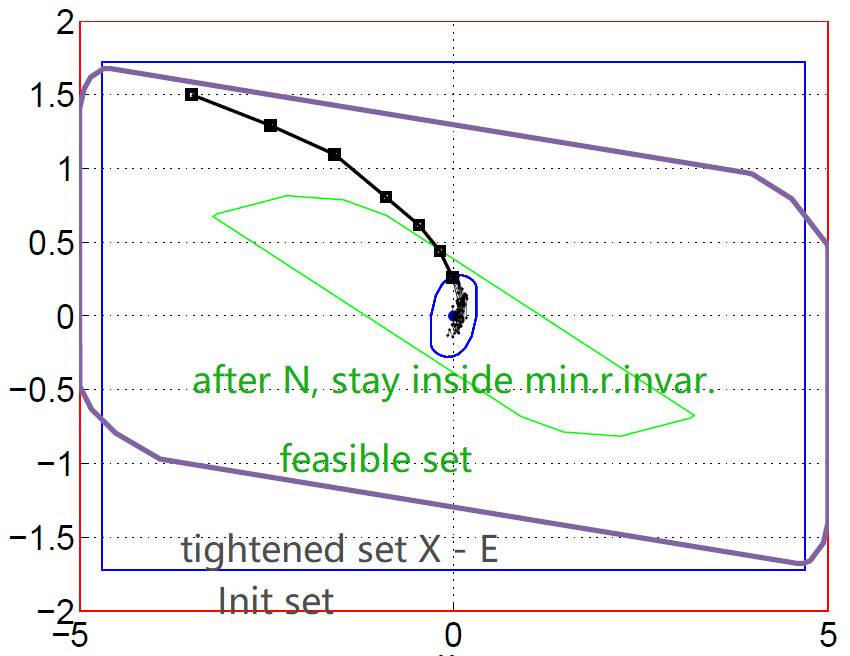
\includegraphics[width=0.65\linewidth]{images/tube3.png}
    \vspace{-5pt}
\end{colfig}

\textbf{Offline:} 1)  Choose \textbf{stabilizing K} such that $ \left\| A + BK \right\| < 1$; 2)\comp minimal robust invariant set $\mathcal{E}=\bigoplus_{k=0}^{\infty} A^{k} \mathbb{W}$ for $x^+ = (Ax + BK)x$; 3)\comp tightened constraints: $\tilde{\mathcal{X}} :=  \mathcal{X} \ominus \mathcal{E}$ and $\tilde{\mathcal{U}} := \mathcal{U} \ominus K\mathcal{E}$; 4) Choose cost and terminal set $\mathcal{X}_f$
	
\textbf{Online:} 1_ Measure/estimate the state $x$; 2) Solve the optimization problem; 3) Apply input $u = \mu_{\mathrm{tube}}(x)$

\quadRule

the system ignoring noise is \textbf{Input-to-State Stable}: Bound that monotonically decreases to $\max\{\Vert w \Vert | w \in \mathbb{W} \}$ (noise size) $\rightarrow$ Converges to $\approx 0$

\section{Explicit MPC}

\textbf{\hl{KKT Conditions} for $\min f(z)$.} %Assume $g_i$ and $h_i$ are differentiable. 
$A$ constraints coeff.; $\lambda$ introduced variables; conditions for optimality:
\begin{enumerate}
    \item Stationarity: $\nabla f(z) + A^{\mathsf{T}}\lambda  = 0$
	\item Primal feasibility: $Az \leq b$, original constraints
	\item Dual feasibility: $\lambda \geq 0$ constraints for $\lambda$
	\item Complementarity: $\lambda^{\mathsf{T}} (Az - b) = 0$
\end{enumerate}
\begin{colfig}
    \centering
    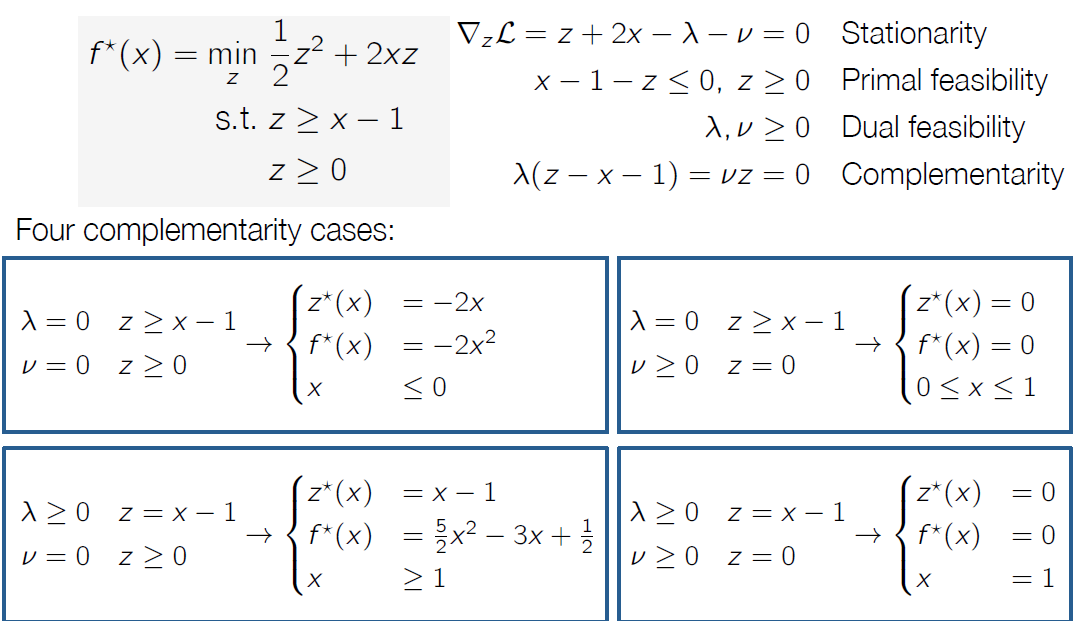
\includegraphics[width=\linewidth]{images/kktExample.png}
    \vspace{-15pt}
\end{colfig}

\comp [$v + (-A^T)\lambda -\nabla f(z)=0$]; [$s + A^Tz = b $]
\comp value $f^*(z)$ by setting (v,s), (z,$\lambda$), (v,$\lambda$) =0
\comp given a q, plot vector $q$ and cheak the cone area from $(e_1, e_2)$ or $(e_2, m_1)$ or $(m_1, m_2)$ or $(m_2, e_1)$ and set others as 0 $\rightarrow$ obtain by $(M-I)^{-1}q$

\quadRule

\textbf{pQP}: $J^{\star}(x):=\min _{u} \frac{1}{2} u^{T} Q u+(F x+f)^{T} u$, s.t.  $G u \geq E x+e,\  u \geq 0$

$\rightarrow$ Parametric Linear Complementarity (\hl{\textbf{pLCP}}): $Iw-M z=Q x+q $; $w, z \geq 0, w^{T} z=0$;
\vspace{-5pt}
\begin{colfig}
    \centering
    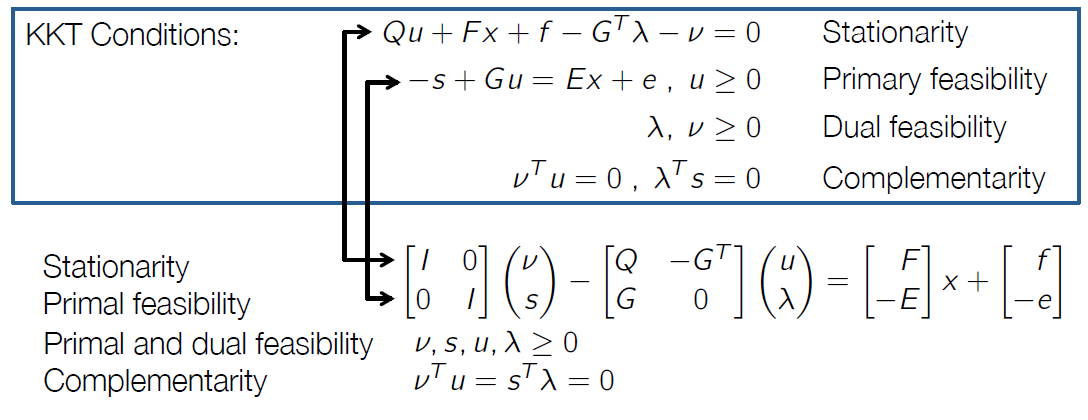
\includegraphics[width=\linewidth]{images/mpcKKT.png}
    \vspace{-16pt}
\end{colfig}

\quadRule

Find cone containing q (critical region): define the polyhedral critical region using the solution $C R(B):=\left\{x \mid A_{B}^{-1}(q+Q x) \geq 0\right\}$

Convex pLCP $\rightarrow$ sufficient matrix $\rightarrow$ 1) unoverlapped cones (unique solution); 2) connected domain (connected neighbour) $\rightarrow$ 
Calculate piecewise affine function and online evaluation $\rightarrow$ Point Location by \textbf{sequential} or \textbf{logarithmic} search

%%%%%% Nonlinear %%%%%% 

\section{Nonlinear MPC}

Nonlinear system $x_{i+1}=f\left(x_{i}, u_{i}\right)$ $\rightarrow$ nonconvex overall cost $\arg\min \sum_{i=0}^{N-1} l\left(x_{i}, u_{i}\right)+V_{f}\left(x_{N}\right)$ while same theory and assumption on feasibility and stability.

\textbf{Challenges}: 1) hard to calculate the invariance set $\rightarrow$  drop the terminal constraints; 2) local minimal

\hl{1) Compute nonconvex $\rightarrow$ descent method}; 
example: Newton's; Gauss-Newton; Sequenctial QP

\hl{2) Discretiziation}: $u(t) = u(t_k) \: \forall t \in \left[ t_k, t_{k+1}\right) $\\
Non-linear: $x(k+1) = x(k) + T_s\cdot g^c(x(k),u(k))$\\
\textbf{Naive}-Euler: $A = I + T_sA^c$ and $B=T_sB^c$\\
Exact: $A=e^{A^c T_s}$ and $B = (A^c)^{-1}(A-I)B^c$
\textbf{Solution:} lin. comb. of initial state and inputs\\ $x(k+N) = A^N x(k) + \sum_{i=0}^{N-1} A^i B u(k+N-1-i)$

\quadRule

Advanced: Direct integration / Collocation

\hl{Runge-Kutta (RK)}-2 as example $x^+ = x(t+h)$

2nd-order Taylor series $x^{+}=x+h \dot{x}+\frac{h^{2}}{2} \ddot{x}+\mathcal{O}\left(h^{3}\right)$
$x^{+} \approx  x+\frac{h}{2} f(x)+\frac{h}{2} f(x+h f(x)) =  x+h\left(\frac{1}{2} k_{1}+\frac{1}{2} k_{2}\right)$ \\
where $k_{1}=f(x)$ and $k_{2}=f\left(x+h k_{1}\right)$

\quadRule

RK4 use higher-order Taylor series $\rightarrow$ high acc.
$
x_{k+1}=x_{k}+h\left(\frac{k_{1}}{6}+\frac{k_{2}}{3}+\frac{k_{3}}{3}+\frac{k_{4}}{6}\right)$, where \\
 $ k_{1}=f\left(t_{k}, x_{k}\right) $, 
$k_{2}=f\left(t_{k}+\frac{h}{2}, x_{k}+\frac{h}{2} k_{1}\right)$, 
$k_{3}=f(t_{k}+\frac{h}{2}, x_{k}+\tfrac{h}{2} k_{2})$, $k_{4}=f\left(t_{k}+h, x_{k}+h k_{3}\right)
$


%%%%%% Exam conclusion %%%%%% 

\section{Remark}
\begin{itemize}
    \item union of a finite set of ellipses \textbf{not necessarily} convex
    \item intersection of an ellipse and a polytope $\rightarrow$ convex
    \item \textbf{symmetric} $Q=Q^T$ and \textbf{nonnegtive eigenvalues} $Q \succeq 0$ (all nonnegtive $\times$) $\rightarrow$ guarante optimization prob $\min x^TQx$ with local $x = x^*$ a \textbf{global} minimum
    \item quadratic function $xTPx$ is convex iff $P$ is PSD.
    
    \quadRule
    
    \item $J^{*}\left(x_{k+1}\right)-J^{*}\left(x_{k}\right) \leq-I\left(x_{k}, u_{0}^{*}\right)$ eusures $J^*(x)$ \hl{Lyapunov function} $\rightarrow$ stability
	\item $\exists$ subset of \hl{pos.invar.} $\neq$ invariant
	\item \textbf{Not} all \hl{pos.invar.} for system $x^+ = f(x)$ can be written as a polyhedron $\{x | G x \leq h\}$
	\item \textbf{intersection} and \textbf{union} of two \hl{pos.invar.} are invar.
	\item \textbf{Convex hull} of \hl{pos.invar.} is invar. if f \textbf{linear}
	\item max.invar. for system is \textbf{union} of given invar.
	
    \quadRule
    
	\item $\exists$ \textbf{possible} that N-step sequence $\in \mathbb{X}$ and MPC controller $\in \mathbb{U}$ given $x_0$ not in \hl{max.ctrl.invar.} $C_{\infty}$
    \item Given $x_0$ in max.\textbf{ctrl}.invar. $C_{\infty}$ for system $f(x,u)$ with constraints $\rightarrow$ $\exists u_0 \in \mathbb{U}$ that $f(x_0, u_0) \notin \mathbb{X}$
    \item $\exists x \in \mathbb{X} $ and $\exists u \in \mathbb{U} $ such that $f(x,u) \in C $ $\iff$
    \textbf{Not} $\exists x \in \mathbb{X}-\{C\} $ and $\exists u \in \mathbb{U} $ such that $f(x,u) \in C $, given same setting before with $(X,S)$
    
    \quadRule
    
    \item $x_s$ always in the interior (boundary $\times$) of invar.
    \item \textbf{No} slack variable weight $\rho$ ensure soft-constrained $J_{\text {soft }}^{\star}(\bar{x})=J^{\star}(\bar{x})$ standard [$\approx$ soft with higher $\rho$]
    
    \quadRule
    
    \item \hl{Minimal \textbf{robust} invar.} $F_{\infty} > \mathbb{X}$ $\rightarrow$ feasible set $\emptyset$
    \item $S \subseteq \operatorname{pre}(S \ominus W)=pre^{\mathbb{W}}(s)$ is invar. of the \textbf{uncertain} system with $w \in \mathbb{W}$
    \item Bounded disturbance syetem $x^{+}=A x+B u+E w$, \hl{max.\textbf{robust} crtl.invar.} $C_{\infty}$ will $= \downarrow$, $= \uparrow$, and $= \downarrow$ after 0.5 $\mathbb{U}$, $\mathbb{W}$, and $\mathbb{X}$
    
    \quadRule
    
    \item MPC value function for all $x$: $J^*(x)$ unconstrained $<=$ constrained infin.hori.ctrl = constrained fin.hori.ctrl w/o terminal $<=$ w.terminal
\end{itemize}


%%%%%%%%%%%%%%%%%%%%%%%%%%%%%%%%%%%%%%%%%%
%% ---------- Credits
\section{Credits}
Most material was taken from the lecture notes of \href{https://edu.epfl.ch/coursebook/fr/model-predictive-control-ME-425}{\textit{Model Predictive Control}} given by \href{https://people.epfl.ch/colin.jones}{\textbf{Prof. Colin Jones
}}.\\
%Cost functions figure from Patrick Breheny's slides.\\
%Biais-variance decomposition figure from Hastie, Tibshirani, Friedman, \textit{The Elements of Statistical Learning}.
%The SVD figure from Kevin P. Murphy, \textit{Machine Learning, A Probabilistic Perspective}.
%
%% ---------- Footer
%\hrule
%\tiny
Written by Yujie He (\texttt{yujie.he@epfl.ch}).

Last Updated and Rendered \today. 

\copyright Yujie He. This work is licensed under the Creative Commons Attribution-ShareAlike 3.0 Unported License.
%To view a copy of this license, visit \href{http://creativecommons.org/licenses/by-sa/3.0/}{http://creativecommons.org/licenses/by-sa/3.0/} or
%send a letter to Creative Commons, 444 Castro Street, Suite 900, Mountain View, California, 94041, USA.
%\includegraphics{images/by-sa.png}
%%%%%%%%%%%%%%%%%%%%%%%%%%%%%%%%%%%%%%%%%%

\end{multicols*}
\end{document}
